\documentclass{mimosis}

\usepackage{metalogo}

%%%%%%%%%%%%%%%%%%%%%%%%%%%%%%%%%%%%%%%%%%%%%%%%%%%%%%%%%%%%%%%%%%%%%%%%
% Some of my favourite personal adjustments
%%%%%%%%%%%%%%%%%%%%%%%%%%%%%%%%%%%%%%%%%%%%%%%%%%%%%%%%%%%%%%%%%%%%%%%%
%
% These are the adjustments that I consider necessary for typesetting
% a nice thesis. However, they are *not* included in the template, as
% I do not want to force you to use them.

% This ensures that I am able to typeset bold font in table while still aligning the numbers
% correctly.
\usepackage{etoolbox}

%%%%%%%%%%%%%%%%%%%%%%%%%%%%%%%%%%%%%%%%%%%%%%%%%%%%%%%%%%%%%%%%%%%%%%%%
% Hyperlinks & bookmarks
%%%%%%%%%%%%%%%%%%%%%%%%%%%%%%%%%%%%%%%%%%%%%%%%%%%%%%%%%%%%%%%%%%%%%%%%

\usepackage[%
  colorlinks = true,
  citecolor  = red,
  linkcolor  = RoyalBlue,
  urlcolor   = RoyalBlue,
  unicode,
  ]{hyperref}

\usepackage{bookmark}
\usepackage{pdfpages}

%%%%%%%%%%%%%%%%%%%%%%%%%%%%%%%%%%%%%%%%%%%%%%%%%%%%%%%%%%%%%%%%%%%%%%%%
% Bibliography
%%%%%%%%%%%%%%%%%%%%%%%%%%%%%%%%%%%%%%%%%%%%%%%%%%%%%%%%%%%%%%%%%%%%%%%%
%
% I like the bibliography to be extremely plain, showing only a numeric
% identifier and citing everything in simple brackets. The first names,
% if present, will be initialized. DOIs and URLs will be preserved.

\usepackage[%
  autocite     = plain,
  backend      = bibtex,
  doi          = true,
  url          = true,
  giveninits   = true,
  hyperref     = true,
  maxbibnames  = 99,
  maxcitenames = 99,
  sortcites    = true,
  style        = numeric,
  ]{biblatex}

\input{bibliography-mimosis}
\addbibresource{thesis.bib}

%%%%%%%%%%%%%%%%%%%%%%%%%%%%%%%%%%%%%%%%%%%%%%%%%%%%%%%%%%%%%%%%%%%%%%%%
% Fonts
%%%%%%%%%%%%%%%%%%%%%%%%%%%%%%%%%%%%%%%%%%%%%%%%%%%%%%%%%%%%%%%%%%%%%%%%

\ifxetexorluatex
  \usepackage{unicode-math}
  \setmainfont{texgyrepagella-regular.otf}[
    BoldFont     = texgyrepagella-bold.otf,
    ItalicFont   = texgyrepagella-italic.otf,
    BoldItalicFont = texgyrepagella-bolditalic.otf
  ]
  \setmathfont{texgyrepagella-math.otf}
  \setmonofont{texgyrecursor-regular.otf}[
    BoldFont     = texgyrecursor-bold.otf,
    ItalicFont   = texgyrecursor-italic.otf,
    BoldItalicFont = texgyrecursor-bolditalic.otf,
    Scale        = MatchLowercase
  ]
\else
  \usepackage{tgpagella}
  \usepackage{tgcursor}
  \singlespacing
\fi

\newacronym[description={Principal component analysis}]{PCA}{PCA}{principal component analysis}
\newacronym                                            {SNF}{SNF}{Smith normal form}
\newacronym[description={Topological data analysis}]   {TDA}{TDA}{topological data analysis}

\newglossaryentry{LaTeX}{%
  name        = {\LaTeX},
  description = {A document preparation system},
  sort        = {LaTeX},
}

\newglossaryentry{Real numbers}{%
  name        = {$\real$},
  description = {The set of real numbers},
  sort        = {Real numbers},
}

\makenoidxglossaries

%%%%%%%%%%%%%%%%%%%%%%%%%%%%%%%%%%%%%%%%%%%%%%%%%%%%%%%%%%%%%%%%%%%%%%%%
% Ordinals
%%%%%%%%%%%%%%%%%%%%%%%%%%%%%%%%%%%%%%%%%%%%%%%%%%%%%%%%%%%%%%%%%%%%%%%%

\makeatletter
\@ifundefined{st}{%
  \newcommand{\st}{\textsuperscript{\textup{st}}\xspace}
}{}
\@ifundefined{rd}{%
  \newcommand{\rd}{\textsuperscript{\textup{rd}}\xspace}
}{}
\@ifundefined{nd}{%
  \newcommand{\nd}{\textsuperscript{\textup{nd}}\xspace}
}{}
\makeatother

\renewcommand{\th}{\textsuperscript{\textup{th}}\xspace}

%%%%%%%%%%%%%%%%%%%%%%%%%%%%%%%%%%%%%%%%%%%%%%%%%%%%%%%%%%%%%%%%%%%%%%%%
% Incipit
%%%%%%%%%%%%%%%%%%%%%%%%%%%%%%%%%%%%%%%%%%%%%%%%%%%%%%%%%%%%%%%%%%%%%%%%

% Set your thesis type: \masterthesistrue or \bachelorthesistrue
% For project reports, leave both false — the academic integrity declaration will be omitted.
\newif\ifmasterthesis
\newif\ifbachelorthesis
% \masterthesistrue  % <-- change this

\title{Your Thesis Title}
\newcommand{\germantitle}{Deutscher Titel der Thesis}
\author{Your Name}

\begin{document}

\frontmatter
  \begin{titlepage}
\makeatletter
\thispagestyle{empty}

{\parindent0pt

\begin{flushright}
  % Replace with your institution's logo in the Cover/ folder:
  
\includegraphics[width=0.4\textwidth]{cover/logoipsum-354}
\end{flushright}

\vspace*{1cm}

{\large
The present work was submitted to the Chair of Computational Science and Engineering.\\

\vspace*{1cm}

presented by / \textcolor{gray}{von} \medskip \\
\@author \medskip \\
\textit{MATRICULATION NUMBER}

\vspace*{1.5cm}

Masterarbeit/Bachelorarbeit/Projektarbeit \medskip \\
\textcolor{gray}{Master's Thesis/Bachelor's Thesis/Project Report} \\
}

\vspace*{1.5cm}

\begin{center}
  {\Large\textbf{\@title}} \\
  \vspace*{5mm}
  {\Large\textcolor{gray}{\germantitle}}
\end{center}

\vspace*{1.5cm}

{\large
Supervisors / \textcolor{gray}{Betreuer}: \medskip \\
FIRST SUPERVISOR \medskip \\
SECOND SUPERVISOR \medskip \\
}

\vfill

{\large
\begin{flushright}
Aachen, \textit{YOUR SUBMISSION DATE}
\end{flushright}
}

}%end parindent0pt

\end{titlepage}

\newpage
\makeatletter
\thispagestyle{empty}

{\parindent0pt
\null\vfill

\begin{center}
  % Replace with a figure representative of your thesis:
  
\includegraphics[width=0.9\textwidth]{images/representative-figure}\\[1cm]
  {\Huge\textbf{\@title}}\\[0.5cm]
  {\large\@author}
\end{center}

\vspace*{2cm}
}

\newpage
\makeatother

  \begin{center}
  \textsc{Abstract}
\end{center}
%
\noindent
%
Write your abstract here. It should briefly summarize the motivation, the problem you address, your approach, and the key results. Aim for around 200--300 words.

  \chapter*{Acknowledgements}

Write your acknowledgements here. Thank your supervisors, colleagues, and anyone else who supported your work. You may also acknowledge funding sources or institutional support.

  \ifmasterthesis
\includepdf[pages=-]{cover/declarationofacademicintegrity}
\else\ifbachelorthesis
\includepdf[pages=-]{cover/declarationofacademicintegrity}
\else

\chapter*{Declaration of Own Work}

I hereby declare that this thesis has been written independently and that no sources other than those cited have been used. All passages taken verbatim or paraphrased from published or unpublished works have been clearly marked as such. This work has not been submitted, in whole or in part, for any other academic qualification.

\fi\fi

\section*{Declaration of AI Tool Usage}

The following AI tools were used during the preparation of this thesis:

\begin{itemize}
  \item \textbf{Tool name} — describe what it was used for (e.g.\ grammar checking, literature search, code generation). Specify which sections or tasks it assisted with.
\end{itemize}

\noindent
All AI-assisted content has been reviewed and verified by the author. No AI tool was used to generate results, draw conclusions, or replace independent scientific reasoning.

\vspace{2cm}

\noindent
Aachen, \textit{YOUR SUBMISSION DATE}

\vspace{1.5cm}

\noindent
\rule{0.4\textwidth}{0.4pt}\\
\textit{Your Name}


  \tableofcontents
  \listoffigures
  \addcontentsline{toc}{chapter}{\listfigurename}
  \listoftables
  \addcontentsline{toc}{chapter}{\listtablename}

  \begingroup
    \let\clearpage\relax
    \glsaddall
    \printnoidxglossary[type=\acronymtype]
    \newpage
    \printnoidxglossary
  \endgroup

  \chapter*{Conventions}
\addcontentsline{toc}{chapter}{Conventions}

This chapter describes the conventions used throughout the thesis to ensure consistency and clarity.

%%%%%%%%%%%%%%%%%%%%%%%%%%%%%%%%%%%%%%%%%%%%%%%%%%%%%%%%%%%%%%%%%%%%%%%%
\section*{Language}

This thesis is written in British/American English.\footnote{Choose one and be consistent throughout.} Technical terms are introduced in \emph{italics} when first used and defined in the Glossary.

%%%%%%%%%%%%%%%%%%%%%%%%%%%%%%%%%%%%%%%%%%%%%%%%%%%%%%%%%%%%%%%%%%%%%%%%
\section*{Notation}

Describe any mathematical or typographical conventions you follow. For example:

\begin{itemize}
  \item Vectors are denoted by bold lowercase letters, e.g.\ $\mathbf{v}$.
  \item Matrices are denoted by bold uppercase letters, e.g.\ $\mathbf{M}$.
  \item Sets are denoted by calligraphic uppercase letters, e.g.\ $\mathcal{S}$.
  \item Scalar variables are denoted by italic letters, e.g.\ $x$.
\end{itemize}

%%%%%%%%%%%%%%%%%%%%%%%%%%%%%%%%%%%%%%%%%%%%%%%%%%%%%%%%%%%%%%%%%%%%%%%%
\section*{References}

Figures, tables, chapters, and sections are referred to with a capital letter, e.g.\ Figure~\ref{fig:design}, Table~\ref{tab:results}, Chapter~\ref{ch:introduction}, Section~\ref{sec:motivation}.


\mainmatter
  \chapter{Introduction}
\label{ch:introduction}

Write your introduction here. A good introduction motivates the problem, states the research questions you aim to answer, and closes with an outline of the thesis structure. Back up important claims with citations.\footnote{A Bachelor's thesis is typically around 50 pages; a Master's thesis around 80 pages. The exact length depends on your programme and the scope of your research.}

%%%%%%%%%%%%%%%%%%%%%%%%%%%%%%%%%%%%%%%%%%%%%%%%%%%%%%%%%%%%%%%%%%%%%%%%
\section{Motivation}
\label{sec:motivation}

Describe the broader context and explain why the problem you are tackling is relevant. What gap in existing work does your thesis address? Why should the reader care?\footnote{Use citations to ground your motivation in the literature. Unsupported claims weaken the introduction.}

%%%%%%%%%%%%%%%%%%%%%%%%%%%%%%%%%%%%%%%%%%%%%%%%%%%%%%%%%%%%%%%%%%%%%%%%
\section{Research Questions}
\label{sec:research-questions}

State the specific research questions or objectives of your thesis. For example:

\begin{itemize}
  \item[\textit{RQ1}] Your first research question.
  \item[\textit{RQ2}] Your second research question.
  \item[\textit{RQ3}] Your third research question.
\end{itemize}

%%%%%%%%%%%%%%%%%%%%%%%%%%%%%%%%%%%%%%%%%%%%%%%%%%%%%%%%%%%%%%%%%%%%%%%%
\section{Outline}
\label{sec:outline}

Briefly describe what each chapter covers. For example:

Chapter~\ref{ch:relatedwork} surveys the existing literature and positions this work within it.
Chapter~\ref{ch:ownwork} presents the approach and its implementation.
Chapter~\ref{ch:evaluation} evaluates the approach against the research questions.
Chapter~\ref{ch:summary} summarises the contributions and outlines directions for future work.

  \chapter{Related Work}
\label{ch:relatedwork}

Present the state of the art relevant to your research questions. This chapter should give the reader enough background to understand your contribution and demonstrate that you are aware of what has already been done.\footnote{If the related work spans multiple distinct domains, organise it into sections — one per domain. This makes the chapter easier to navigate.}

When citing, integrate author names naturally into your sentences when presenting their work, rather than appending citations as afterthoughts. For example: ``Smith et al.\ showed that \ldots~[1]''.

To find relevant publications, use academic search engines and domain-specific libraries.\footnote{%
  General: Google Scholar, Scopus, Web of Science, Semantic Scholar.
  Computer science: ACM Digital Library, IEEE Xplore, arXiv (preprints).
  Engineering \& sciences: ScienceDirect (Elsevier), SpringerLink, ASME Digital Collection, ASCE Library, PLOS.
  Natural sciences: PubMed, Web of Science.
  Open-source software: Journal of Open Source Software (JOSS), Journal of Open Research Software (JORS).
  Prefer peer-reviewed conference and journal papers over web sources. Use footnotes for web links and \texttt{\textbackslash cite} for articles, books, and papers.}

%%%%%%%%%%%%%%%%%%%%%%%%%%%%%%%%%%%%%%%%%%%%%%%%%%%%%%%%%%%%%%%%%%%%%%%%
\section{Topic Area One}
\label{sec:related-topic-one}

Summarise the key works in the first relevant area. Highlight what they contribute and where they fall short with respect to your problem.

%%%%%%%%%%%%%%%%%%%%%%%%%%%%%%%%%%%%%%%%%%%%%%%%%%%%%%%%%%%%%%%%%%%%%%%%
\section{Topic Area Two}
\label{sec:related-topic-two}

Summarise the key works in the second relevant area. End the chapter by making clear how your thesis builds on and differs from the existing literature.

  \chapter{Your Contribution}
\label{ch:ownwork}

Replace the chapter title above with a descriptive name for your main contribution. This is the core chapter of your thesis — it should present your approach, design, or system in enough detail that a reader could reproduce or build upon it.\footnote{If your contribution has multiple distinct components, consider splitting this into more than one chapter.}

%%%%%%%%%%%%%%%%%%%%%%%%%%%%%%%%%%%%%%%%%%%%%%%%%%%%%%%%%%%%%%%%%%%%%%%%
\section{Hypotheses}
\label{sec:hypotheses}

If your work is hypothesis-driven, state your hypotheses clearly here. For example:

\begin{itemize}
  \item[\textit{H1}] Your first hypothesis.
  \item[\textit{H2}] Your second hypothesis.
  \item[\textit{H3}] Your third hypothesis.
\end{itemize}

%%%%%%%%%%%%%%%%%%%%%%%%%%%%%%%%%%%%%%%%%%%%%%%%%%%%%%%%%%%%%%%%%%%%%%%%
\section{Approach}
\label{sec:approach}

Describe your approach, design, or methodology. Explain the decisions you made and justify them. Figures and tables should be used to support your explanation.

\subsection{Design}
\label{sec:design}

Describe the design of your system, study, or method. A figure is often the best way to convey an architecture or workflow:

\begin{figure}[ht]
  \centering
  % Replace with your own figure in the Images/ folder:
  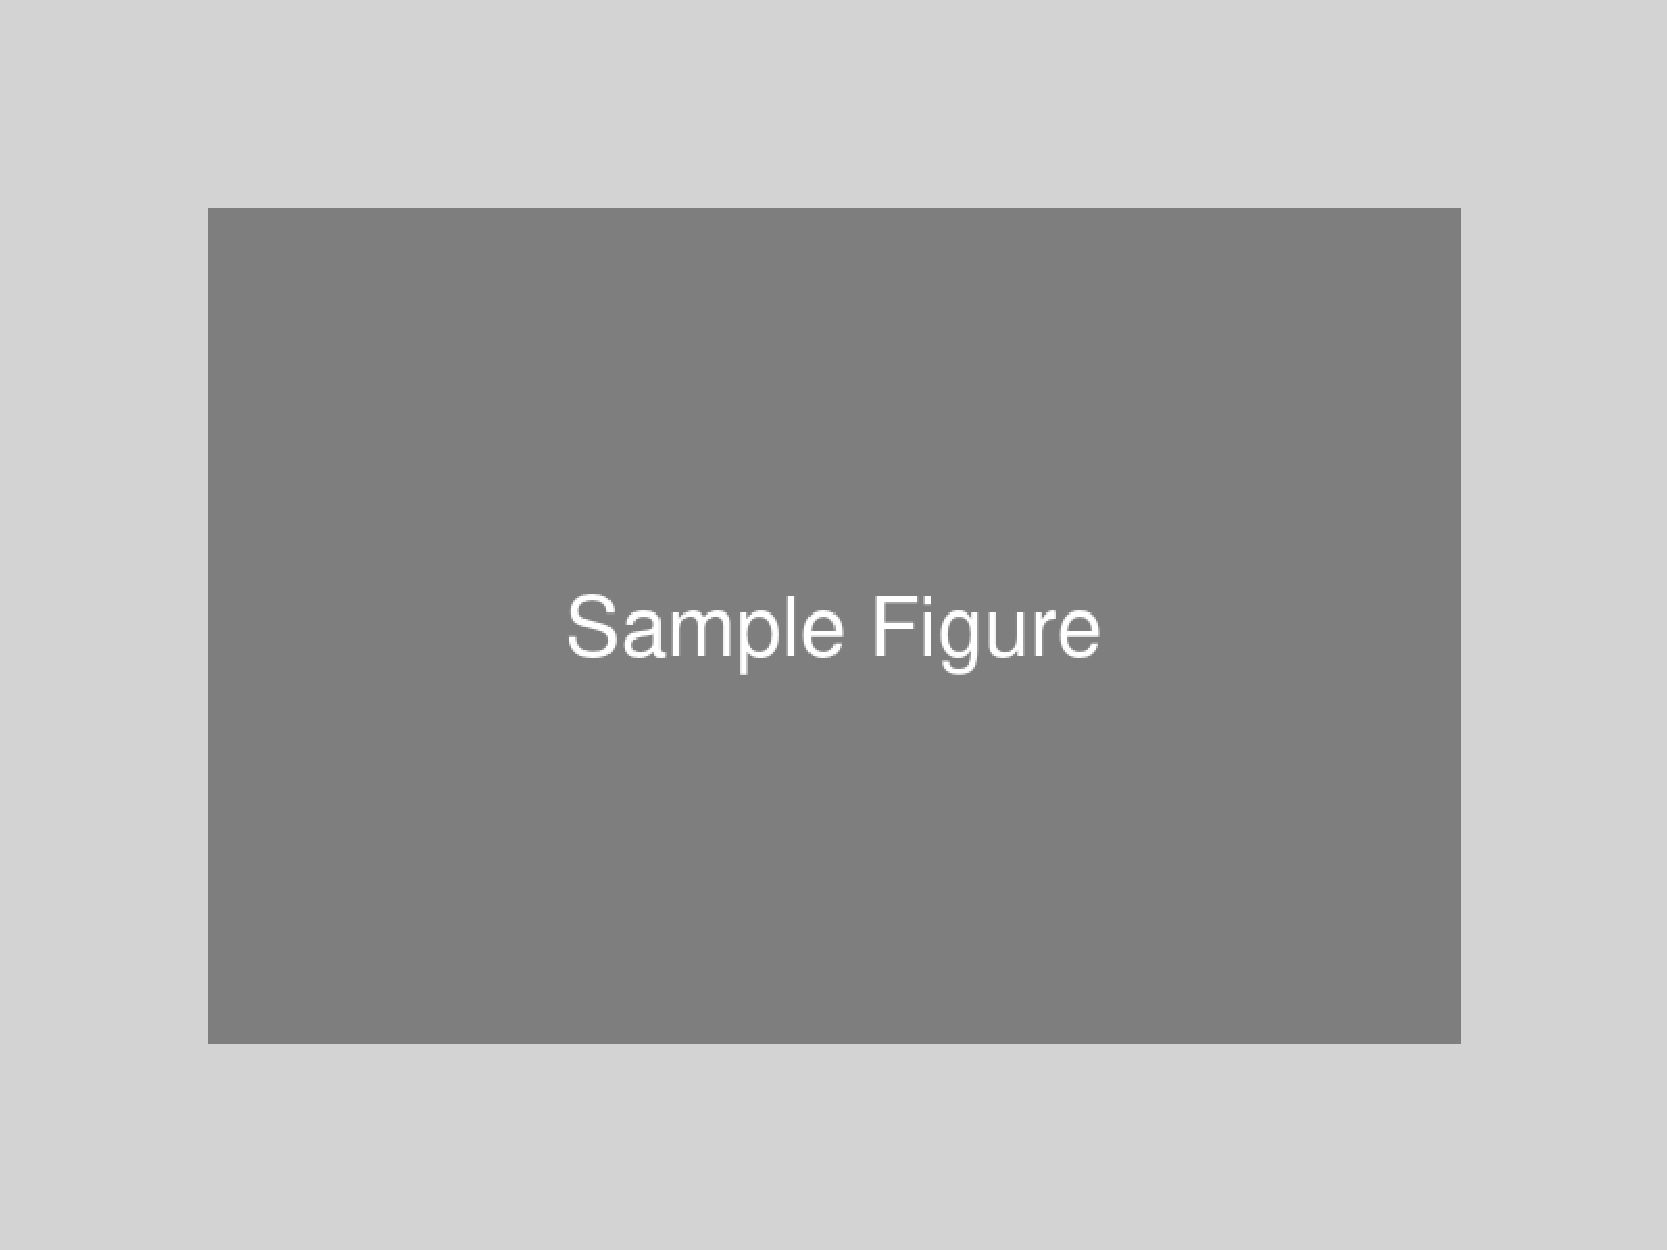
\includegraphics[width=0.8\textwidth]{images/sample-figure}
  \caption{A caption describing what the figure shows.}
  \label{fig:design}
\end{figure}

\subsection{Mathematical Formulation}
\label{sec:math}

If your approach involves a mathematical formulation, present it here. Use numbered equations for anything you refer to later in the text:

\begin{equation}
  f(x) = \frac{1}{\sigma\sqrt{2\pi}} \exp\left(-\frac{(x - \mu)^2}{2\sigma^2}\right)
  \label{eq:example}
\end{equation}

For multiple related equations, use the \texttt{align} environment to align them at the equals sign:

\begin{align}
  \mu    &= \frac{1}{N} \sum_{i=1}^{N} x_i \\
  \sigma &= \sqrt{\frac{1}{N} \sum_{i=1}^{N} (x_i - \mu)^2}
\end{align}

Refer to equations by number in the text, e.g.\ Equation~\eqref{eq:example}.

\subsection{Implementation}
\label{sec:implementation}

Describe any relevant implementation details — tools, frameworks, datasets, or parameters used.\footnote{Be precise: include version numbers, dataset sizes, and hardware specs where relevant so that your work is reproducible.}

%%%%%%%%%%%%%%%%%%%%%%%%%%%%%%%%%%%%%%%%%%%%%%%%%%%%%%%%%%%%%%%%%%%%%%%%
\section{Results}
\label{sec:results}

Present your results objectively. Use tables and figures to summarise findings, and refer to them explicitly in the text.

\begin{table}[ht]
  \centering
  \begin{tabular}{lcc}
    \toprule
    \textbf{Condition} & \textbf{Metric A} & \textbf{Metric B} \\
    \midrule
    Baseline  & 0.00 & 0.00 \\
    Your method & 0.00 & 0.00 \\
    \bottomrule
  \end{tabular}
  \caption{Summary of results. Cells contain mean values.}
  \label{tab:results}
\end{table}

%%%%%%%%%%%%%%%%%%%%%%%%%%%%%%%%%%%%%%%%%%%%%%%%%%%%%%%%%%%%%%%%%%%%%%%%
\section{Discussion}
\label{sec:discussion}

Interpret your results in the context of your research questions and hypotheses. What do the findings mean? Where does your approach succeed and where does it fall short?\footnote{Be honest about limitations — a well-reasoned discussion of weaknesses is a sign of scientific maturity.}

  \chapter{Evaluation}
\label{ch:evaluation}

This chapter evaluates your contribution against the research questions stated in Chapter~\ref{ch:introduction}. Define clear evaluation criteria before presenting results — what does success look like?\footnote{A good evaluation is systematic: it states what is being measured, how, and why that measure is meaningful.}

%%%%%%%%%%%%%%%%%%%%%%%%%%%%%%%%%%%%%%%%%%%%%%%%%%%%%%%%%%%%%%%%%%%%%%%%
\section{Experimental Setup}
\label{sec:experimental-setup}

Describe the conditions under which your evaluation was conducted. Include datasets, baselines, metrics, and any relevant hardware or software configuration.\footnote{Be precise enough that someone else could replicate your evaluation.}

%%%%%%%%%%%%%%%%%%%%%%%%%%%%%%%%%%%%%%%%%%%%%%%%%%%%%%%%%%%%%%%%%%%%%%%%
\section{Metrics}
\label{sec:metrics}

Define the metrics you use to assess your approach. Explain why each metric is appropriate for your research questions.

%%%%%%%%%%%%%%%%%%%%%%%%%%%%%%%%%%%%%%%%%%%%%%%%%%%%%%%%%%%%%%%%%%%%%%%%
\section{Results}
\label{sec:eval-results}

Present the evaluation results. Use tables and figures to summarise comparisons across conditions or baselines.

\begin{table}[ht]
  \centering
  \begin{tabular}{lcc}
    \toprule
    \textbf{Method} & \textbf{Metric A} & \textbf{Metric B} \\
    \midrule
    Baseline   & 0.00 & 0.00 \\
    Your method & 0.00 & 0.00 \\
    \bottomrule
  \end{tabular}
  \caption{Comparison of your method against the baseline across evaluation metrics.}
  \label{tab:eval-results}
\end{table}

%%%%%%%%%%%%%%%%%%%%%%%%%%%%%%%%%%%%%%%%%%%%%%%%%%%%%%%%%%%%%%%%%%%%%%%%
\section{Discussion}
\label{sec:eval-discussion}

Interpret the evaluation results. Do they support your hypotheses? Where does your approach perform well and where does it struggle? Relate findings back to the research questions.\footnote{If results are mixed or negative, discuss why — this is valuable scientific contribution in itself.}

  \chapter{Summary and Future Work}
\label{ch:summary}

Briefly restate the problem you addressed and summarise how your work contributes to solving it. This chapter should give a reader who skips to the end a clear picture of what was done and what comes next.

%%%%%%%%%%%%%%%%%%%%%%%%%%%%%%%%%%%%%%%%%%%%%%%%%%%%%%%%%%%%%%%%%%%%%%%%
\section{Summary}
\label{sec:summary}

Revisit your research questions from Chapter~\ref{ch:introduction} and state concisely how each was addressed. Highlight your key contributions.\footnote{Avoid simply repeating the abstract — this section should reflect on the work as a whole, now that the reader has seen all the details.}

\begin{itemize}
  \item[\textit{RQ1}] How your first research question was answered.
  \item[\textit{RQ2}] How your second research question was answered.
  \item[\textit{RQ3}] How your third research question was answered.
\end{itemize}

%%%%%%%%%%%%%%%%%%%%%%%%%%%%%%%%%%%%%%%%%%%%%%%%%%%%%%%%%%%%%%%%%%%%%%%%
\section{Limitations}
\label{sec:limitations}

Discuss the boundaries of your work — what assumptions were made, what was out of scope, and what threats to validity exist.\footnote{Acknowledging limitations honestly strengthens rather than weakens your thesis.}

%%%%%%%%%%%%%%%%%%%%%%%%%%%%%%%%%%%%%%%%%%%%%%%%%%%%%%%%%%%%%%%%%%%%%%%%
\section{Future Work}
\label{sec:future-work}

Identify open questions and promising directions that follow from your work. What would you do differently with more time? What problems does your work open up that did not exist before?


\appendix
  \chapter{Supplementary Material}
\label{app:supplementary}

Include here any material that supports the main text but would disrupt the flow of the thesis if placed inline. Typical appendix content includes raw data, additional figures, extended tables, questionnaires, or code listings.\footnote{Only include material that is genuinely referenced from the main text. An appendix is not a dump for unused work.}

%%%%%%%%%%%%%%%%%%%%%%%%%%%%%%%%%%%%%%%%%%%%%%%%%%%%%%%%%%%%%%%%%%%%%%%%
\chapter{Additional Figures and Tables}
\label{app:figures-tables}

Place additional figures and tables here that were omitted from the main chapters for brevity but are referenced in the text.


% This ensures that the subsequent sections are being included as root
% items in the bookmark structure of your PDF reader.
\bookmarksetup{startatroot}
\backmatter
  \printbibliography

\end{document}
